\documentclass[../main/main.tex]{subfiles}
\begin{document}

\chapter{Dipôles et associations}\label{ch:O1}
\vspace*{-47pt}

\begin{center}
    \Huge Exercices d'application
\end{center}

\section{Circuit simple}\label{ch2:ex1}
\begin{center}
    \begin{NCdefi}[width=.5\linewidth]{Données}
        Générateur \underline{réel} $(E,r)$ de tension : \smallbreak
        \begin{center}
            \begin{circuitikz}[scale=1]
                \draw
                (0,0) node {$\bullet$}
                    to[V]
                (2,0) to[R, name=r]
                (4,0) node {$\bullet$};
                \node[] at (r.center) {$r$};
            \end{circuitikz}
        \end{center}
    \end{NCdefi}
\end{center}

\subsection{}
\begin{tcbraster}[raster columns=3, raster equal height=rows]
    \begin{NCprop}{Résultat attendu}
        On demande un schéma \underline{normalisé}, autrement dit avec les
        conventions de schémas \textit{européennes}.
    \end{NCprop}
    \begin{NCdemo}{Outils}
        Générateur :
        \begin{circuitikz}
            \draw
            (0,0) to[V]
            (2,0) ;
        \end{circuitikz} \smallbreak
        Résistance :\vspace{12pt}
        \begin{circuitikz}
            \draw
            (0,0) to[R, name=R]
            (2,0) ;
            \node[] at (R.center) {$R$};
        \end{circuitikz}
    \end{NCdemo}
    \begin{NCcexe}{Application}
        On obtient : \smallbreak
        \begin{circuitikz}
            \draw
            (0,0)
                to[V]
            (2,0) to[R, name=r]
            (4,0) --
            (4,-2) to[R, name=R]
            (0,-2) -- (0,0);
            \node[] at (r.center) {$r$};
            \node[] at (R.center) {$R$};
        \end{circuitikz}
    \end{NCcexe}
\end{tcbraster}

\ctikzset{voltage/distance from node=.1}
\subsection{}
\begin{tcbraster}[raster columns=2, raster equal height=rows]
    \begin{NCdemo}{Outils}
        Générateur convention générateur : \smallbreak
        \vspace{-12pt}
        \begin{center}
            \begin{circuitikz}
                \draw
                (0,0) to[V, name=E, V^>=$E_{}$, i^>=$I_{}$, !vi]
                (2,0) ;
                \varronly{E} \iarronly{E}
            \end{circuitikz} 
        \end{center}
        Résistance convention récepteur : \smallbreak
        \vspace{-12pt}
        \begin{center}
            \begin{circuitikz}
                \draw
                (0,0) to[R, name=R, i>^=$i$, v^<=$U_R$, !vi]
                (2,0) ;
                \varronly{R} \iarronly{R}
                \node[] at (R.center) {$R$};
            \end{circuitikz}
        \end{center}
    \end{NCdemo}
    \begin{NCexem}{Application}
        \begin{center}
            \begin{circuitikz}
                \draw
                (0,0)
                    to[V, name=E, V^>=$E_{}$, i^>=$I_{}$, !vi]
                (2,0) to[R, name=r, v^<=$U_{r}$, !vi]
                (4,0) --
                (4,-2) -- (3,-2)
                    to[R, name=R, i>_=$I$, v^<=$U_R$, !vi]
                (1,-2) -- (0,-2) -- (0,0);
                \iarronly{E} \varronly{E} \varronly{r} \varronly{R} \iarronly{R}
                \node[] at (r.center) {$r$};
                \node[] at (R.center) {$R$};
            \end{circuitikz} 
        \end{center}
    \end{NCexem}
\end{tcbraster}

\newpage
\subsection{}
\begin{tcbraster}[raster columns=5, raster equal height=rows]
    \begin{NCprop}[raster multicolumn=2]{Résultat attendu}
        À partir d'un circuit où on considère $E$, $r$ et $R$ comme des
        grandeurs connues, on cherche l'intensité $I$ qui parcourt la maille que
        l'on vient de tracer.
    \end{NCprop}
    \begin{NCrema}[raster multicolumn=3]{Remarque}
        Il y a deux outils qui seront utiles pour déterminer des grandeurs dans
        des circuits : la \textbf{loi des mailles} et la \textbf{loi des nœuds}.
        À cela se rajoute la \textbf{loi d'Ohm} qui relie tension et intensité
        dans une résistance. Ces notions seront vues dans le chapitre suivant et
        donc décrites ultérieurement, on va ici utiliser la compositon des
        tensions.
    \end{NCrema}
\end{tcbraster}
\begin{tcbraster}[raster columns=3, raster equal height=rows]
    \begin{NCdemo}{Outil}
        En nommant des points d'intérêt du circuit, ce qui est souvent
        conseillé, on va pouvoir utiliser la composition $U_\mathrm{AC} =
        U_\mathrm{AB} + U_\mathrm{BC}$ en respectant le sens des tensions pour
        obtenir une information supplémentaire sur le circuit. \smallbreak
        On rappelle que deux points sur un fil sont au même potentiel, et on
        peut donc les nommer de la même manière.
    \end{NCdemo}
    \begin{NCexem}[raster multicolumn=2, sidebyside]{Application}
        \tcbsubtitle[before skip=\baselineskip,
        colback = darkgray!50!black,
        colframe = darkgray!50!black]{Schéma}
        \begin{center}
            \begin{circuitikz}
                \draw
                (0,0) node {$\bullet$} node [above left, ForestGreen] {A}
                    to[V, name=E, V^>=$E_{}$, i^>=$I_{}$, !vi]
                (2,0) node {$\bullet$} node [below, ForestGreen] {B}
                    to[R, name=r, v^<=$U_{r}$, !vi]
                (4,0) node {$\bullet$} node [above right, ForestGreen] {C} --
                (4,-2) node {$\bullet$} node [below right, ForestGreen] {C} --
                (3,-2)
                    to[R, name=R, i>_=$I$, v^<=$U_R$, !vi]
                (1,-2) --
                (0,-2) node {$\bullet$} node [below left, ForestGreen] {A} --
                (0,0);
                \iarronly{E} \varronly{E} \varronly{r} \varronly{R} \iarronly{R}
                \node[] at (r.center) {$r$};
                \node[] at (R.center) {$R$};
            \end{circuitikz} 
        \end{center}
        \tcblower
        \tcbsubtitle[before skip=\baselineskip,
        colback = darkgray!50!black,
        colframe = darkgray!50!black]{Calcul}
        Ici on peut écrire
        \begin{align*}
            U_\mathrm{AB} + U_\mathrm{BC} + U_\mathrm{CA} & = U_\mathrm{AA}\\
            \Leftrightarrow -E + U_r + U_R                & = 0
        \end{align*}
        et avec la \textbf{loi d'Ohm}, i.e. $U_r = rI$ et $U_R = RI$ :
        \begin{equation*}
            (r+R)I = E\\
        \end{equation*}
        soit
        \begin{equation*}
            \boxed{I = \frac{E}{r+R}}
        \end{equation*}
    \end{NCexem}
\end{tcbraster}

\subsection{}
\begin{tcbraster}[raster columns=2, raster equal height=rows]
    \begin{NCdemo}{Outil}
        Pour un récepteur de tension $U$ traversé par l'intensité $I$ en
        convention récepteur, la puissance absorbée est \fbox{$P=UI$}.
    \end{NCdemo}
    \begin{NCexem}{Application}
        Ici, la tension aux bornes de $R$ est $U_R = RI$, avec $I$ l'intensité
        la traversant. On a donc
        \begin{equation*}
            \boxed{P_R = RI^2 = \frac{RE^2}{(r+R)^2}}
        \end{equation*}
    \end{NCexem}
\end{tcbraster}

\subsection{}
\begin{tcbraster}[raster columns=3, raster equal height=rows]
    \begin{NCprop}{Résultat attendu}
        On cherche à faire une étude de la fonction $P$ de variable $R$, comme
        on ferait l'étude de $f(x)$ en mathématiques.
    \end{NCprop}
    \begin{NCdemo}[raster multicolumn=2]{Outils}
        Bon sens pour l'allure de la courbe, procédés de dérivation pour le
        maximum. D'une manière générale, on a besoin de :
        \begin{itemize}
            \item Dérivation d'un produit :
                \begin{equation*}
                    \boxed{D[\textcolor{Purple!70}{u}
                        \textcolor{orange}{v}] =
                    \textcolor{brandeisblue}{u'}\textcolor{orange}{v} +
                \textcolor{Red!70}{v'}\textcolor{Purple!70}{u}}
                \end{equation*}
            \item Dérivation d'une fonction $u$ élevée à une puissance $\alpha$
                :
                \begin{equation*}
                    \boxed{D[\textcolor{Purple}{u}^
                        {\textcolor{ForestGreen}{\alpha}}] =
                    \textcolor{ForestGreen}{\alpha} \textcolor{brandeisblue}{u'}
                \textcolor{Purple}{u}^{\textcolor{Goldenrod}{\alpha-1}}}
                \end{equation*}
        \end{itemize}
    \end{NCdemo}
\end{tcbraster}
\vfill
\begin{NCexem}[breakable, sidebyside, righthand width=.58\linewidth]{Application}
    \tcbsubtitle[before skip=\baselineskip,
    colback = darkgray!50!black,
    colframe = darkgray!50!black]{Tracé}
    \hspace{-12pt}
    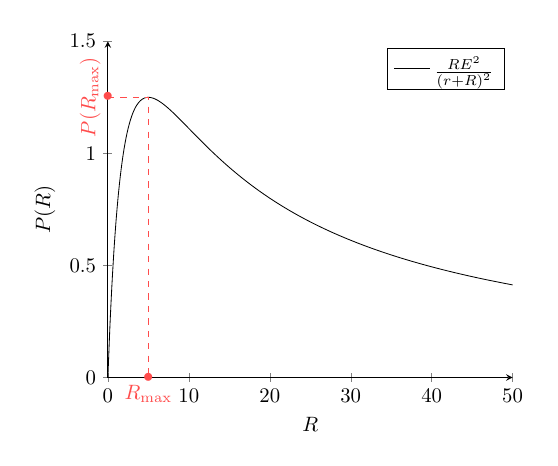
\begin{tikzpicture}[scale=0.75]
        \def\E{5}
        \def\r{5}
        \begin{axis}[
            axis lines=left,
            xmin=0, xmax=50,
            ymin=0, ymax=1.5,
            xlabel=$R$, ylabel=$P(R)$,
            clip=false]
            \addplot[
                domain=0:50,
                samples=200,
                smooth]
                {x*\E^2/(\r+x)^2};
                \addlegendentry{$\frac{RE^2}{(r+R)^2}$}
            \draw[dashed, Red!70]
            (0,1.25) node {$\bullet$} node [above, rotate=90]
            {$P(R_\mathrm{max})$} --++
            (5,0) --++
            (0,-1.25) node {$\bullet$} node[below] {$R_\mathrm{max}$};
        \end{axis}
    \end{tikzpicture}
    \tcblower
    \tcbsubtitle[before skip=\baselineskip,
    colback = darkgray!50!black,
    colframe = darkgray!50!black]{Calcul}
    Soit
    \begin{itemize}
        \item $ \left\{\begin{array}{rcl}
                    \textcolor{orange}{v} : \Rb^+ & \rightarrow & \Rb^+\\
                    R                             & \mapsto     & \DS \textcolor{orange}{R}\\
            \end{array}\right.\quad\quad\hspace{0.7em}\Longrightarrow
            \left\{\begin{array}{rcl}
                    \textcolor{Red}{v'} : \Rb^+ & \rightarrow & \Rb^+\\
                    R                           & \mapsto     & \DS \textcolor{Red}{1}\\
            \end{array}\right.$
        \item $ \left\{\begin{array}{rcl}
                    \textcolor{Purple}{u} : \Rb^+ & \rightarrow & \Rb^+\\
                    R                             & \mapsto     & \DS \textcolor{Purple}{r+R}\\
            \end{array}\right.\quad\hspace{0.5em}\Longrightarrow
            \left\{\begin{array}{rcl}
                    \textcolor{brandeisblue}{u'} : \Rb^+ & \rightarrow & \Rb^+\\
                    R                                    & \mapsto     & \DS \textcolor{brandeisblue}{1}\\
            \end{array}\right.$
    \end{itemize}
    Ainsi
    \begin{itemize}
        \item $ \left\{\begin{array}{rcl}
                    \textcolor{Purple}{u}^{\textcolor{ForestGreen}{{-2}}} : \Rb^+ & \rightarrow & \Rb^+\\
                    R              & \mapsto     &
                    \frac{\textcolor{ForestGreen}{1}}{\textcolor{Purple}{(r+R)}^{\textcolor{ForestGreen}{2}}}\\
            \end{array}\right.\Longrightarrow
            \left\{\begin{array}{rcl}
                    D[\textcolor{Purple}{u}^{\textcolor{ForestGreen}{{-2}}}] : \Rb^+ & \rightarrow & \Rb^-\\
                    R                 & \mapsto     &
                    \frac{\textcolor{ForestGreen}{-2}\times\textcolor{brandeisblue}{1}}
                    {\textcolor{Purple}{(r+R)}^{\textcolor{Goldenrod}{3}}}\\
            \end{array}\right.$
    \end{itemize}
    Et donc,
    \begin{align*}
        P'(R) & = \frac{\textcolor{ForestGreen}{-2}}
        {\textcolor{Purple}{(r+R)}^{\textcolor{Goldenrod}{3}}}
        \times \textcolor{orange}{R} + \textcolor{Red}{1}\times
        \frac{\textcolor{ForestGreen}{1}}
        {\textcolor{Purple}{(r+R)}^{\textcolor{ForestGreen}{2}}}\\
        P'(R) & = \frac{-2R}{(r+R)^3} + \frac{r+R}{(r+R)^3}
    \end{align*}
    Ainsi
    \begin{equation*}
        \boxed{P'(R) = \frac{r-R}{(r+R)^3}}
    \end{equation*}
    Et donc
    \begin{equation*}
        P'(R_\mathrm{max}) = 0 \Longrightarrow
        \textcolor{Red!70}{\boxed{R_\mathrm{max} = r}}
    \end{equation*}
    Avec
    \begin{equation*}
        \textcolor{Red!70}{\boxed{P(R_\mathrm{max}) = \frac{E^2}{4r}}}
    \end{equation*}
\end{NCexem}

\section{Résistances équivalentes}
\subsection{}
\begin{tcbraster}[raster columns=2, raster equal height=rows]
    \begin{NCprop}{Résultat attendu}
        \begin{center}
            \begin{circuitikz}[scale=1]
                \draw
                (0.5,0) node {$\bullet$} node [left] (A) {A} --
                (1,0) coordinate (Il) --
                (1,0.5) to[R, name=R1]
                (3,0.5) --
                (3,0) coordinate (Ir) --
                (3.5,0) node {$\bullet$} node [right] (B) {B};
                \draw[]
                (Il) --
                (1,-0.5) to[R, name=R2]
                (3,-0.5) -- (Ir);
                \node[] at (R1.center) {$R_1$};
                \node[] at (R2.center) {$R_2$};
                \node[right=0.7em] (E) at (B) {$\equiv$};
                \draw[shift={($(E)+(2em,0)$)}]
                (0,0) node[left] {A} node {$\bullet$}
                to[R, name=Req]
                (2,0) node {$\bullet$} node [right] {B};
                \node[] at (Req.center) {$R_{\rm eq}$};
            \end{circuitikz}
        \end{center}
    \end{NCprop}
    \begin{NCdemo}{Outil}
        L'association en parallèle de deux résistances $R_1$ et $R_2$ donne une
        résistance équivalente $ R_{\rm eq}$ telle que :
        \begin{empheq}[box=\fbox]{equation*}
            \frac{1}{ R_{\rm eq}} = \frac{1}{R_1} + \frac{1}{R_2}
        \end{empheq}
    \end{NCdemo}
    \begin{NCimpo}{Attention !}
        Faites particulièrement attention à bien écrire $\DS \frac{1}{ R_{\rm
        eq}}$ et non pas simplement $ R_{\rm eq}$, même après 5 lignes de calcul
        quand c'est nécessaire. Pensez toujours à vérifier l'homogénéité d'un
        résultat littéral avant de l'encadrer. Cette erreur est une des plus
        communes.
    \end{NCimpo}
    \begin{NCexem}{Application}
        En mettant les deux termes sur même dénominateur :
        \begin{align*}
            \frac{1}{ R_{\rm eq}} & = \frac{1}{R_1}\times \textcolor{orange}{
            \frac{R_2}{R_2}} + \frac{1}{R_2}\times \textcolor{orange}{
        \frac{R_1}{R_1}} \\
         \Leftrightarrow \frac{1}{ R_{\rm eq}} & = \frac{R_2 + R_1}{R_1R_2}\\
         \Leftrightarrow R_{\rm eq}            & = \frac{R_1R_2}{R_1+R_2}
        \end{align*}
    \end{NCexem}
\end{tcbraster}

\subsection{}
\begin{center}
    \begin{NCexem}[width=.5\linewidth]{Application}
        \[R_1 = R_2 = R \Longrightarrow \boxed{ R_{\rm eq} = \frac{R}{2}}\]
    \end{NCexem}
\end{center}

\subsection{}
\begin{tcbraster}[raster columns=2, raster equal height=rows]
    \begin{NCprop}{Résultat attendu}
        \begin{center}
            \begin{circuitikz}[scale=1]
                \draw
                (0.5,0) node {$\bullet$} node [left] (A) {A} --
                (1,0) coordinate (Il) --
                (1,0.7) to[R, name=R1]
                (3,0.7) --
                (3,0) coordinate (Ir) --
                (3.5,0) node {$\bullet$} node [right] (B) {B};
                \draw[]
                (Il) --
                (1,-0.7) to[R, name=R3]
                (3,-0.7) -- (Ir);
                \draw[] 
                (Il) to[R, name=R2]
                (Ir);
                \node[] at (R1.center) {$R_1$};
                \node[] at (R2.center) {$R_2$};
                \node[] at (R3.center) {$R_3$};
                \node[right=0.7em] (E) at (B) {$\equiv$};
                \draw[shift={($(E)+(2em,0)$)}]
                (0,0) node[left] {A} node {$\bullet$}
                to[R, name=Req]
                (2,0) node {$\bullet$} node [right] {B};
                \node[] at (Req.center) {$R_{\rm eq}$};
            \end{circuitikz}
        \end{center}
    \end{NCprop}
    \begin{NCdemo}{Outil}
        L'association en parallèle de trois résistances $R_1$, $R_2$ et $R_3$
        donne une résistance équivalente $ R_{\rm eq}$ telle que :
        \begin{empheq}[box=\fbox]{equation*}
            \frac{1}{ R_{\rm eq}} = \frac{1}{R_1} + \frac{1}{R_2} + \frac{1}{R_3}
        \end{empheq}
    \end{NCdemo}
\end{tcbraster}
\begin{center}
    \begin{NCexem}[width=.5\linewidth]{Application}
        De la même manière que précédemment, la mise sous même dénominateur
        donne :
        \begin{align*}
            \frac{1}{ R_{\rm eq}} & = \frac{R_2R_3}{R_1R_2R_3} +
            \frac{R_1R_3}{R_1R_2R_3} + \frac{R_1R_2}{R_1R_2R_3}\\
            \Leftrightarrow R_{\rm eq} & = \frac{R_1R_2R_3}{R_1R_2 + R_2R_3 +
            R_1R_3}
        \end{align*}
        qui est bien homogène à une résistance étant de la forme $\DS
        \frac{R^{\cancel{3}}}{\cancel{R^2}} = R$.
    \end{NCexem}
\end{center}

\subsection{}
\begin{center}
    \begin{NCexem}[width=.5\linewidth]{Application}
        \[R_1 = R_2 = R_3 = R \Longrightarrow R_{\rm eq} = \frac{R^3}{3R^2}
        \Leftrightarrow \boxed{R_{\rm eq} = \frac{R}{3}}\]
    \end{NCexem}
\end{center}

\subsection{}
\begin{tcbraster}[raster columns=2, raster equal height=rows]
    \begin{NCprop}{Résultat attendu}
        \begin{center}
            \begin{circuitikz}[scale=1]
                \draw
                (0.5,0) node {$\bullet$} node [left] (A) {A} --
                (1,0) coordinate (Il) --
                (1,0.7) to[R, name=R1]
                (3,0.7) --
                (3,0) coordinate (Ir) --
                (3.5,0) node {$\bullet$} node [right] (B) {B};
                \draw[]
                (Il) --++ (0,-0.2) coordinate (Ilf);
                \draw[dashed] 
                (Ilf) --++ (0,-1) coordinate (Ild);
                \draw[] 
                (Ild) --
                (1,-1.4) to[R, name=R3]
                (3,-1.4) -- (3,-1.2) coordinate (Ird);
                \draw[dashed]
                (Ird) --++ (0,1) coordinate (Irf);
                \draw[]
                (Irf) -- (Ir);
                \draw[] 
                (Il) to[R, name=R2]
                (Ir);
                \node[] at (R1.center) {$R$};
                \node[] at (R2.center) {$R$};
                \node[] at (R3.center) {$R$};
                \node[below=0.5] (text) at (R2.center) {\textit{n fois}};
                \node[right=0.7em] (E) at (B) {$\equiv$};
                \draw[shift={($(E)+(2em,0)$)}]
                (0,0) node[left] {A} node {$\bullet$}
                to[R, name=Req]
                (2,0) node {$\bullet$} node [right] {B};
                \node[] at (Req.center) {$R_{\rm eq}$};
            \end{circuitikz}
        \end{center}
    \end{NCprop}
    \begin{NCexem}{Application}
        Il n'y a toujours qu'une seule formule attendue, et elle s'écrit :
        \[ \frac{1}{R_{\rm eq}} = \underbrace{ \frac{1}{R} + \frac{1}{R} +
            \cdots + \frac{1}{R}}_{\textit{n fois}} \Leftrightarrow
        \boxed{R_{\rm eq} = \frac{R}{n}} \]
    \end{NCexem}
\end{tcbraster}

\newpage
\section{Association de générateurs}\label{ch2:ex3}
\titleformat{\subsection}{\color{brandeisblue}\bfseries}{\hspace{-0.3em}
\arabic{section}) \Alph{subsection}-}{.5em}{}{}
\titleformat{\subsubsection}{\color{capri}\bfseries}{\hspace{-0.3em}
\arabic{section}) \Alph{subsection}- \arabic{subsubsection}.}{.5em}{}{}

\subsection{Générateurs en série}
\begin{tcbraster}[raster columns=5, raster equal height=rows]
    \begin{NCdefi}[raster multicolumn=2]{Schéma}
        \subsubsection{}\vspace*{-20pt}
        \begin{center}
            \begin{circuitikz}
                \draw
                (0,0)
                to[V, name=E1, V^>=$E_{1}$, i^>=$i_{1}$, !vi]
                (0,2)
                to[R, name=r1, i_>=$i_1$, v^<=$U_{r_1}$, !vi]
                (0,4)
                to[V, name=E2, V^>=$E_{2}$, i_>=$i_2$, !vi]
                (2,4)
                to[R, name=r2, v^<=$U_{r_2}$, !vi]
                (4,4) --
                (4,3)
                to[R, name=R3, i>^=$i$, v^<=$U_{R_3}$, !vi]
                (4,1) --
                (4,0) --
                (0,0);
                \varronly{E1} \varronly{r1} \varronly{r2} \varronly{E2}
                \varronly{R3}
                \iarronly{E1} \iarronly{r1} \iarronly{E2} \iarronly{R3}
                \node[] at (r1.center) {$r_1$};
                \node[] at (r2.center) {$r_2$};
                \node[] at (R3.center) {$R_3$};
                \node[Orchid, scale=2] (LM1) at (2,2) {1};
                \circledarrow{Orchid, thick}{(LM1)}{0.5};
            \end{circuitikz}    
        \end{center}
    \end{NCdefi}
    \begin{NCdemo}[raster multicolumn=3]{Outil}
        %\vspace{-12pt}
        \subsubsection{}
        \textbf{Loi des mailles} : la somme algébrique des tensions d'une maille
        est nulle (cf. exercice \ref{ch2:ex1}). Pour l'appliquer, on se donne un
        sens de lecture d'une maille, ici dans le sens direct mais peu importe,
        puis on peut :
        \begin{itemize}
            \item Écrire les tensions traversées dans le même sens que leur
                flèche d'un côté du signe égal, les autres de l'autre côté ;
            \item Écrire les tensions traversées dans le même sens avec un «~+~»
                et les autres avec un «~-~», le tout devant «~$=0$~».
        \end{itemize}
    \end{NCdemo}
\end{tcbraster}
\begin{tcbraster}[raster columns=9, raster equal height=rows]
    \begin{NCexem}[raster multicolumn=4]{Application}
        Étant donné qu'il n'y a qu'une maille, il ne peut y avoir qu'une seule
        intensité dans le circuit. On pose donc $i_1 = i_2 = i$, et en applicant
        la loi des mailles on a
        \begin{align*}
            & U_{R_3} + U_{r_2} - E_2 + U_{r_1} - E_1 =
                0\\
            & \Leftrightarrow R_3i + r_2i + r_1i =
                E_1 + E_2
                \quad\quad \mathrm{\textbf{Loi d'Ohm}}\\
            & \Leftrightarrow i \left( r_1+r_2+R_3 \right) =
                E_1 + E_2\\
            & \Leftrightarrow \boxed{i = \frac{E_1 + E_2}{r_1+r_2+R_3}}
        \end{align*}
    \end{NCexem}    
    \begin{NCimpl}[raster multicolumn=5]{Schéma simplifié}
        \subsubsection{}
        L'expression que l'on a trouvée est en tout point similaire à celle du
        premier exercice si on considère qu'on a un générateur de force
        électromagnétique $E = E_1 + E_2$ et de résistance interne $r = r_1 +
        r_2$ ; on peut donc dessiner :
        \begin{center}
            \begin{circuitikz}
                \draw
                (0,0)
                    to[V, name=E, V^>=$E_{}$, i^>=$i_{}$, !vi]
                (2,0) to[R, name=r, v^<=$U_{r}$, !vi]
                (4,0) --
                (4,-2) -- (3,-2)
                to[R, name=R3, i>_=$i$, v^<=$U_{R_3}$, !vi]
                (1,-2) -- (0,-2) -- (0,0);
                \iarronly{E} \varronly{E} \varronly{r}
                \varronly{R3} \iarronly{R3}
                \node[] at (r.center) {$r$};
                \node[] at (R3.center) {$R_3$};
            \end{circuitikz} 
        \end{center}
    \end{NCimpl}
\end{tcbraster}
\begin{tcbraster}[raster columns=2, raster equal height=rows]
    \begin{NCcoro}{Situation particulière}
        \subsubsection{}
        Quand $r_1$ et $r_2$ sont nulles, on se retrouve avec un générateur de
        résistance interne $r = 0$ : c'est donc un \underline{générateur idéal}.
    \end{NCcoro}
    \begin{NCimpo}{Conclusion}
        L'étude théorique précédente ne présente aucune incohérence ou
        impossibilité de pratique peu importe la situation, si tant est que les
        générateurs sont branchés dans le même sens ; si ça n'est pas le cas
        l'un considère l'autre comme un récepteur et le fait surchauffer.
    \end{NCimpo}
\end{tcbraster}

\subsection{Générateurs en parallèle}
\begin{tcbraster}[raster columns=5, raster equal height=rows]
    \begin{NCdefi}[raster multicolumn=2]{Schéma}
        \subsubsection{}
        \vspace*{-12pt}
        \begin{center}
            \begin{circuitikz}
                \draw
                (0,0)
                to[V, name=E1, V^>=$E_{1}$, i^>=$i_{1}$, !vi]
                (0,2)
                to[R, name=r1, i_>=$i_1$, v^<=$U_{r_1}$, !vi]
                (0,4) --
                (2,4) coordinate (N1)
                to[R, name=r2, i<^=$i_2$, v^>=$U_{r_2}$, !vi]
                (2,2)
                to[V, name=E2, V^<=$E_{2}$, i<_=$i_{2}$, !vi]
                (2,0) coordinate (N2) --
                (0,0);
                \draw[]
                (N1) --++
                (2,0) --++
                (0,-1)
                to[R, name=R4, i>^=$i_3$, v^<=$U_{R_4}$, !vi]
                (4,1) --
                (4,0) --
                (N2);
                \varronly{E1} \varronly{r1} \varronly{r2} \varronly{E2}
                \varronly{R4}
                \iarronly{E1} \iarronly{r1} \iarronly{r2} \iarronly{E2}
                \iarronly{R4}
                \node[] at (r1.center) {$r_1$};
                \node[] at (r2.center) {$r_2$};
                \node[] at (R4.center) {$R_4$};
            \end{circuitikz} 
        \end{center}
    \end{NCdefi}
    \begin{NCexem}[raster multicolumn=3]{Générateurs idéaux}
        \subsubsection{}\vspace*{-20pt}
        \begin{center}
            \begin{circuitikz}
                \draw
                (0,0)
                    node {$\bullet$}
                    node [below left] {B}
                to[V, name=E1, V^>=$E_{1}$, i^>=$i_{1}$, !vi]
                (0,2)
                    node {$\bullet$}
                    node [above] {A} --
                (2,2) coordinate (N1)
                    node {$\bullet$}
                    node [above right] {A}
                to[V, name=E2, V^<=$E_{2}$, i<_=$i_{2}$, !vi]
                (2,0) coordinate (N2)
                    node {$\bullet$}
                    node [below] {B} --
                (0,0);
                \draw[]
                (N1) --
                (4,2)
                    node {$\bullet$}
                    node [above right] {A}
                to[R, name=R4, i>^=$i$, v^<=$U_{R_4}$, !vi]
                (4,0)
                    node {$\bullet$}
                    node [below right] {B} --
                (N2);
                \varronly{E1} \varronly{E2}
                \varronly{R4}
                \iarronly{E1} \iarronly{E2}
                \iarronly{R4}
                \node[] at (R4.center) {$R_4$};
            \end{circuitikz} 
        \end{center}
        On doit trouver (avec l'unicité de la tension entre deux points, ici par
        exemple A et B) que $U_{R_4} = E_2 = E_1$.
    \end{NCexem}
\end{tcbraster}
\begin{center}
    \begin{NCcexe}[width=.5\linewidth]{Conclusion}
        On ne peut brancher des générateurs idéaux de tension que si leurs
        tensions sont les mêmes ; les générateurs réels peuvent l'être et ce
        sont les intensités qui vont s'adapter pour suivre la loi des mailles.
    \end{NCcexe}
\end{center}

\titleformat{\subsection}{\color{brandeisblue}\bfseries}{\hspace{-0.3em}
\arabic{section}) \arabic{subsection}-}{.5em}{}{}
\titleformat{\subsubsection}{\color{capri}\bfseries}{\hspace{-0.3em}
\arabic{section}) \arabic{subsection}- \alph{subsubsection}.}{.5em}{}{}
\section{Calculs de résistances équivalentes}
On retrouve la forme de l'exercice \ref{ch1:ex4}. On va donc procéder de la même
manière en trouvant les résistances équivalentes que l'on peut déterminer (soit
en série, soit en dérivation), en faisant le schéma correspondant, puis en
déterminant les nouvelles relations qui en découlent.

\subsection{Schéma 1}
\begin{center}
    \begin{circuitikz}
        \draw
        (0,0) node {$\bullet$} node [left] (A) {A}
        to[R, name=R1]
        (2,0) coordinate (N1) %node [above] {N1}
        to[R, name=R2]
        (4,0)
        to[R, name=R3 ]
        (4,-2) coordinate (Nbr) --
        (2,-2) coordinate (N2) %node [below] {N2}
        to[R, name=R4]
        (0,-2) node {$\bullet$} node [left] (B) {B};
        \draw[] 
        (N1)
        to[R, name=R5]
        (N2);
        \foreach \n in {1, 2, ..., 5}{
            \node[] at (R\n.center) {$R$};}
        \draw[dashed, ForestGreen]
        ([shift={(0.3,0.3)}]N1) rectangle
        ([shift={(0.3,-0.3)}]Nbr);
        \node[right=1em] (E1) at (R3) {$\equiv$};
        \draw[shift={($(E1)+(2em,1)$)}]
        (0,0) node {$\bullet$} node [left] (A) {A}
        to[R, name=R1]
        (2,0) coordinate (N1) -- %node [above] {N1}
        (4,0)
        to[R, name=Req1, color=ForestGreen]
        (4,-2) coordinate (Nbr) --
        (2,-2) coordinate (N2) %node [below] {N2}
        to[R, name=R2]
        (0,-2) node {$\bullet$} node [left] (B) {B};
        \draw[] 
        (N1)
        to[R, name=R3]
        (N2);
        \foreach \n in {1, 2, 3}{
            \node[] at (R\n.center) {$R$};}
        \node[rotate=90] at (Req1.center) {\color{ForestGreen} $R_{\rm eq,1}$};
        \draw[dashed, brandeisblue]
        ([shift={(-0.3,0.3)}]N1) rectangle
        ([shift={(0.3,-0.3)}]Nbr);        
        \node[right=1em] (E2) at (Req1) {$\equiv$};
        \draw[shift={($(E2)+(2em,1)$)}]
        (0,0) node {$\bullet$} node [left] (A) {A}
        to[R, name=R1, color=orange]
        (2,0) coordinate (N1)
        to[R, name=Req2, color=brandeisblue]
        (2,-2) coordinate (Nbr)
        to[R, name=R2, color=orange]
        (0,-2) node {$\bullet$} node [left] (B) {B};
        \node[] at (R1.center) {\color{orange}$R$};
        \node[] at (R2.center) {\color{orange}$R$};
        \node[rotate=90] at (Req2.center) {\color{brandeisblue} $R_{\rm eq,2}$};
        \node[right=1em] (E3) at (Req2) {$\equiv$};
        \draw[shift={($(E3)+(2em,0)$)}]
        (0,0) node {$\bullet$} node [left] {A}
        to[R, name=Req]
        (2,0) node {$\bullet$} node [right] {B};
        \node[] at (Req.center) {$ R_{\rm eq}$};
    \end{circuitikz}
\end{center}
La suite de schémas équivalents précédents donne :
\begin{align*}
    R_{\rm eq}                 & = \textcolor{orange}{R + R} +
        \textcolor{brandeisblue}{R_{\rm eq,2}} \\
    \Leftrightarrow R_{\rm eq} & = \textcolor{orange}{2R} +
        \textcolor{brandeisblue}{\frac{
                R\times \textcolor{ForestGreen}{R_{\rm eq,1}}
        }{R + \textcolor{ForestGreen}{R_{\rm eq,1}}}}\\
    \Leftrightarrow R_{\rm eq} & = 2R + \frac{
        R\times\textcolor{ForestGreen}{2R}}{
        R+\textcolor{ForestGreen}{2R}} \\
    \Leftrightarrow R_{\rm eq} & = 2R + \frac{2R^{\cancel{2}}}{3\cancel{R}}\\
    \Leftrightarrow R_{\rm eq} & = \frac{8R}{3}
\end{align*}

\subsection{}
\begin{center}
    \begin{circuitikz}
        \draw
        (0,0) node {$\bullet$} node [left] (A) {A}
        to[R, name=R1]
        (2,0) coordinate (N1) %node [above] {N1}
        to[R, name=R]
        (4,0)
        to[R, name=R2r]
        (4,-2) coordinate (Nbr)
        to[R, name=r, !vi]
        (2,-2) coordinate (N2) -- %node [below] {N2}
        (0,-2) node {$\bullet$} node [left] (B) {B};
        \draw[] 
        (N1)
        to[R, name=R2l]
        (N2);
        \node[] at (R1.center) {$R_1$};
        \node[] at (R.center) {$R$};
        \node[] at (R2r.center) {$R_2$};
        \node[] at (R2l.center) {$R_2$};
        \node[] at (r.center) {$r$};
        \draw[dashed, ForestGreen]
        ([shift={(0.3,0.3)}]N1) rectangle
        ([shift={(0.3,-0.3)}]Nbr);
        \node[right=1em] (E1) at (R2r) {$\equiv$};
        \draw[shift={($(E1)+(2em,1)$)}]
        (0,0) node {$\bullet$} node [left] (A) {A}
        to[R, name=R1]
        (2,0) coordinate (N1) --%node [above] {N1}
        (4,0)
        to[R, name=Req1, color=ForestGreen]
        (4,-2) coordinate (Nbr) --
        (2,-2) coordinate (N2) -- %node [below] {N2}
        (0,-2) node {$\bullet$} node [left] (B) {B};
        \draw[] 
        (N1)
        to[R, name=R2l]
        (N2);
        \node[] at (R1.center) {$R_1$};
        \node[] at (R2l.center) {$R_2$};
        \node[rotate=90] at (Req1.center) {\color{ForestGreen}$R_{\rm eq,1}$};
        \draw[dashed, brandeisblue]
        ([shift={(-0.3,0.3)}]N1) rectangle
        ([shift={(0.3,-0.3)}]Nbr);        
        \node[right=1em] (E2) at (Req1) {$\equiv$};
        \draw[shift={($(E2)+(2em,1)$)}]
        (0,0) node {$\bullet$} node [left] (A) {A}
        to[R, name=R1, color=orange]
        (2,0) coordinate (N1)
        to[R, name=Req2, color=brandeisblue]
        (2,-2) coordinate (Nbr) --
        (0,-2) node {$\bullet$} node [left] (B) {B};
        \node[] at (R1.center) {\color{orange}$R_1$};
        \node[rotate=90] at (Req2.center) {\color{brandeisblue}$R_{\rm eq,2}$};
        \node[right=1em] (E3) at (Req2) {$\equiv$};
        \draw[shift={($(E3)+(2em,0)$)}]
        (0,0) node {$\bullet$} node [left] {A}
        to[R, name=Req]
        (2,0) node {$\bullet$} node [right] {B};
        \node[] at (Req.center) {$ R_{\rm eq}$};
    \end{circuitikz}
\end{center}
Et cette fois :
\begin{align*}
    R_{\rm eq}                 & =
    \textcolor{orange}{R_1} + \color{brandeisblue}R_{\rm eq,2} \\
    \Leftrightarrow R_{\rm eq} & =
        R_1 + \textcolor{brandeisblue}{\frac{
        R_2\times \textcolor{ForestGreen}{R_{\rm eq,1}}}{
        R_2 + \textcolor{ForestGreen}{R_{\rm eq,1}}}} \\
    \Leftrightarrow R_{\rm eq} & =
        R_1 + \frac{R_2\times(r+R+R_2)}{r+R+2R_2}\\
\end{align*}

\subsection{}
Ce schéma est un peu plus compliqué, mais la bonne pratique de nommer des points
de potentiel sur un schéma aide à ne pas se perdre. En effet, étant donné que
l'on nous demande de déterminer la résistance équivalente entre A et B, toute
simplification du circuit est à faire. On a travaillé sur les associations de
résistances mais il ne faut pas oublier, et donc savoir reconnaître, les
potentiels court-circuits. Ici, en reportant le point A sur chaque point
d'intérêt où il peut être reporté (c'est-à-dire s'il n'y a pas de dipôle entre
les deux), on voit qu'un courant qui partirait de A pour aller à B (ce que fait
un Ohmmètre) éviterait complètement les trois premières résistances. On peut
redessiner le schéma différemment pour faire apparaître le court-circuit de
manière plus explicite :

\begin{center}
    \begin{circuitikz}
        \draw
        (0,0)
            node {\color{Purple}$\bullet$}
            node [above left] {\color{Purple}A}
        to[R, name=R1l, !vi]
        (2,0) coordinate (N1)
            node {\color{brandeisblue}$\bullet$}
            node [above] {\color{brandeisblue}C}
        to[R, name=R1m, !vi]
        (4,0) coordinate (N2)
            node {\color{Rhodamine}$\bullet$}
            node [above] {\color{Rhodamine}A}
        to[R, name=R1r, !vi]
        (6,0)
            node {\color{red}$\bullet$}
            node [above right] {\color{red}B}
        to[R, name=R2r, !vi]
        (6,-2)
            node {\color{Rhodamine}$\bullet$}
            node [below] {\color{Rhodamine}A}
        to[short, name=Sbr, i<=$i$, !vi]
        (4,-2) coordinate (N3)
            node {\color{orange}$\bullet$}
            node [below] {\color{orange}A}
        to[short, name=Sbm, i<=$i$, !vi]
        (2,-2) coordinate (N4)
            node {\color{ForestGreen}$\bullet$}
            node [below] {\color{ForestGreen}A}
        to[short, name=Sbl, i<=$i$, !vi]
        (0,-2)
            node {$\bullet$}
            node [below left] {A}
        to[short, name=Sl, i<=$i$, !vi]
        (0,0);
        \iarronly{Sl}\iarronly{Sbl}\iarronly{Sbm}\iarronly{Sbr}
        \draw
        (N1)
        to[R, name=R2l, !vi]
        (N4);
        \draw[]
        (N2)
        to[short, name=Sr, i<=$i$, !vi]
        (N3);
        \iarronly{Sr}
        \foreach \n in {l,m,r}{
            \node[] at (R1\n.center) {$R_1$};}
        \foreach \n in {l,r}{
            \node[] at (R2\n.center) {$R_2$};}
        \node[right=1em] (E) at (R2r.center) {$\equiv$};
        \draw[shift={($(E)+(2em,-0.5)$)}]
        (0,0)
            node {$\bullet$}
            node [above left] {A} --
		(0.5,0) --
		(0.5,1)
            node {$\bullet$}
            node [above left] {A} --
		(1,1) --
		(1,1.5)
            node {\color{Purple}$\bullet$}
            node [above left] {\color{Purple}A}
        to[R, name=R1l]
		(3,1.5) --
        (3,1)
            node {\color{brandeisblue}$\bullet$}
            node [left] {\color{brandeisblue}C}
        to[R, name=R1m]
		(5,1)
            node {\color{Rhodamine}$\bullet$}
            node [above right] {\color{Rhodamine}A} --
		(5,0)
        to[short, name=Sm, i>=$i$]
		(6,0) --
        (6,0.5)
            node {\color{Rhodamine}$\bullet$}
            node [above left] {\color{Rhodamine}A}
        to[R, name=R1r]
		(8,0.5) --
		(8,0) --
		(8.5,0)
            node {\color{red}$\bullet$}
            node [right] {\color{red}B};
		\draw[shift={($(E)+(2em,-0.5)$)}] (0.5,0) --
		(0.5,-0.5)
            node {\color{ForestGreen}$\bullet$}
            node [below left] {\color{ForestGreen}A}
        to[short, name=Sb, i>=$i$]
		(5,-0.5)
            node {\color{orange}$\bullet$}
            node [below right] {\color{orange}A} --
		(5,0);
		\draw[shift={($(E)+(2em,-0.5)$)}]
        (1,1) --
		(1,0.5)
            node {\color{ForestGreen}$\bullet$}
            node [below left] {\color{ForestGreen}A}
        to[R, name=R2l]
		(3,0.5) --
		(3,1);
		\draw[shift={($(E)+(2em,-0.5)$)}]
        (6,0) --
        (6,-0.5)
            node {\color{Rhodamine}$\bullet$}
            node [below left] {\color{Rhodamine}A}
        to[R, name=R2r]
		(8,-0.5) --
		(8,0);
        \iarronly{Sb} \iarronly{Sm}
        \foreach \n in {l,m,r}{
            \node[] at (R1\n.center) {$R_1$};}
        \foreach \n in {l,r}{
            \node[] at (R2\n.center) {$R_2$};}
    \end{circuitikz}
\end{center}

Ainsi, le circuit se simplifie en :
\begin{center}
    \begin{circuitikz}[scale=1]
        \draw
        (0.5,0) node {$\bullet$} node [left] (A) {A} --
        (1,0) coordinate (Il) --
        (1,0.5) to[R, name=R1]
        (3,0.5) --
        (3,0) coordinate (Ir) --
        (3.5,0) node {$\bullet$} node [right] (B) {B};
        \draw[]
        (Il) --
        (1,-0.5) to[R, name=R2]
        (3,-0.5) -- (Ir);
        \node[] at (R1.center) {$R_1$};
        \node[] at (R2.center) {$R_2$};
        \node[right=0.7em] (E) at (B) {$\equiv$};
        \draw[shift={($(E)+(2em,0)$)}]
        (0,0) node[left] {A} node {$\bullet$}
        to[R, name=Req]
        (2,0) node {$\bullet$} node [right] {B};
        \node[] at (Req.center) {$R_{\rm eq}$};
    \end{circuitikz}
\end{center}
Soit
\[ \boxed{R_{\rm eq} = \frac{R_1R_2}{R_1 + R_2}}\]

\section{Conventions}
\begin{center}
    \begin{NCrapp}[width=.7\linewidth]{Rappel}
        Dans une maille d'un circuit, les puissances fournies et reçues
        s'équilibrent, ce qui se traduit par $\DS \sum P_{\text{fournies}} =
        \sum P_{\text{reçues}}$, avec les conventions :
        \begin{tabularx}{\linewidth}{|Y*{2}{|Y}|}\hline
            &
            Dipôle \textcolor{ForestGreen}{récepteur} &
            Dipôle \textcolor{CornflowerBlue}{générateur}
            \\\hline
            Convention récepteur
            \smallbreak $\textcolor{orange}{P_{\text{reçue}}}$ &
            \begin{circuitikz}
                \draw
                (0,0)
                to[R, name=R, i^<=$i$, v^>=$U$, !vi]
                (2,0);
                \varronly{R} \iarronly{R}
                \node[below] at (R.south)
                    {$\textcolor{orange}{P_{\text{reçue}}}
                    \textcolor{ForestGreen}{> 0}$};
            \end{circuitikz} &
            \begin{circuitikz}
                \draw
                (0,0)
                to[V, name=E, i^<=$i$, V^>=$U$, !vi]
                (2,0);
                \varronly{E} \iarronly{E}
                \node[below] at (R.south)
                    {$\textcolor{orange}{P_{\text{reçue}}}
                    \textcolor{CornflowerBlue}{< 0}$};
            \end{circuitikz}
            \\\hline
            Convention générateur
            \smallbreak $\textcolor{Purple}{P_{\text{fournie}}}$ &
            \begin{circuitikz}
                \draw
                (0,0)
                to[R, name=R, i^>=$i$, v^>=$U$, !vi]
                (2,0);
                \varronly{R} \iarronly{R}
                \node[below] at (R.south)
                    {$\textcolor{Purple}{P_{\text{fournie}}}
                    \textcolor{ForestGreen}{< 0}$};
            \end{circuitikz} &
            \begin{circuitikz}
                \draw
                (0,0)
                to[V, name=E, i^>=$i$, V^>=$U$, !vi]
                (2,0);
                \varronly{E} \iarronly{E}
                \node[below] at (R.south)
                    {$\textcolor{Purple}{P_{\text{fournie}}}
                    \textcolor{CornflowerBlue}{> 0}$};
            \end{circuitikz}
            \\\hline
        \end{tabularx}
    \end{NCrapp}
\end{center}
    
\subsection{Tout récepteur}
\begin{tcbraster}[raster columns=3, raster equal height=rows]
    \begin{NCdefi}{Schéma}
        \subsubsection{}
        \vfill
        \begin{center}
            \begin{circuitikz}
                \draw
                (0,0)
                to[V, name=E, V^>=$E_{}$, i^<=$I_{}$, !vi]
                (0,2)
                to[R, name=r, i^<=$I$, v^>=$U_r$, !vi]
                (2,2)
                to[R, name=R, i^<=$I$, v^>=$U_R$, !vi]
                (2,0) --
                (0,0);
                \varronly{E} \varronly{r} \varronly{R}
                \iarronly{E} \iarronly{r} \iarronly{R}
                \node[] at (r.center) {$r$};
                \node[] at (R.center) {$R$};
            \end{circuitikz}
        \end{center}
        \vfill
    \end{NCdefi}
    \begin{NCdemo}{Calcul préliminaire}
        \subsubsection{}
        \vfill
        \begin{itemize}
            \item $P_{\text{reçue}}(E) = -EI$
            \item $P_{\text{reçue}}(r) = rI^2$
            \item $P_{\text{reçue}}(R) = RI^2$
        \end{itemize}
        \vfill
    \end{NCdemo}
    \begin{NCexem}{Application}
        \subsubsection{}
        On a $\DS \sum P_{\text{fournies}} = \sum P_{\text{reçues}}$ : en
        convention récepteur, il n'y a pas de puissances fournies, donc d'après
        la question précédente :
        \begin{align*}
            0         & = -EI + rI^2 + RI^2\\
            I(r+R)    & = E\\
            \Aboxed{I & = \frac{E}{r+R}}
        \end{align*}
    \end{NCexem}
\end{tcbraster}

\subsection{Tout générateur}
\begin{tcbraster}[raster columns=3, raster equal height=rows]
    \begin{NCdefi}{Schéma}
        \subsubsection{}
        \vfill
        \begin{center}
            \begin{circuitikz}
                \draw
                (0,0)
                to[V, name=E, V^>=$E_{}$, i^>=$I_{}$, !vi]
                (0,2)
                to[R, name=r, i^>=$I$, v^>=$U_r$, !vi]
                (2,2)
                to[R, name=R, i^>=$I$, v^>=$U_R$, !vi]
                (2,0) --
                (0,0);
                \varronly{E} \varronly{r} \varronly{R}
                \iarronly{E} \iarronly{r} \iarronly{R}
                \node[] at (r.center) {$r$};
                \node[] at (R.center) {$R$};
            \end{circuitikz}
        \end{center}
        \vfill
    \end{NCdefi}
    \begin{NCdemo}{Calcul préliminaire}
        \subsubsection{}
        \vfill
        \begin{itemize}
            \item $P_{\text{fournie}}(E) = EI$
            \item $P_{\text{fournie}}(r) = -rI^2$
            \item $P_{\text{fournie}}(R) = -RI^2$
        \end{itemize}
        \vfill
    \end{NCdemo}
    \begin{NCexem}{Application}
        \subsubsection{}
        On a $\DS \sum P_{\text{fournies}} = \sum P_{\text{reçues}}$ : en
        convention générateur, il n'y a pas de puissances reçues, donc d'après
        la question précédente :
        \begin{align*}
            EI - rI^2 - RI^2 & = 0\\
            I(r+R)           & = E\\
            \Aboxed{I        & = \frac{E}{r+R}}
        \end{align*}
    \end{NCexem}
\end{tcbraster}

\subsection{Conventions combinées}
\begin{tcbraster}[raster columns=3, raster equal height=rows]
    \begin{NCdefi}{Schéma}
        \subsubsection{}
        \vfill
        \begin{center}
            \begin{circuitikz}
                \draw
                (0,0)
                to[V, name=E, V^>=$E_{}$, i^>=$I_{}$, !vi]
                (0,2)
                to[R, name=r, i^>=$I$, v^<=$U_r$, !vi]
                (2,2)
                to[R, name=R, i^>=$I$, v^<=$U_R$, !vi]
                (2,0) --
                (0,0);
                \varronly{E} \varronly{r} \varronly{R}
                \iarronly{E} \iarronly{r} \iarronly{R}
                \node[] at (r.center) {$r$};
                \node[] at (R.center) {$R$};
            \end{circuitikz}
        \end{center}
        \vfill
    \end{NCdefi}
    \begin{NCdemo}{Calcul préliminaire}
        \subsubsection{}
        \vfill
        \begin{itemize}
            \item $P_{\text{fournie}}(E) = EI$
            \item $P_{\text{reçue}}(r) = rI^2$
            \item $P_{\text{reçue}}(R) = RI^2$
        \end{itemize}
        \vfill
    \end{NCdemo}
    \begin{NCexem}{Application}
        \subsubsection{}
        On a $\DS \sum P_{\text{fournies}} = \sum P_{\text{reçues}}$ : avec les
        conventions adaptées à chaque dipôle, on a :
        \begin{align*}
            EI        & = rI^2 + RI^2\\
            I(r+R)    & = E\\
            \Aboxed{I & = \frac{E}{r+R}}
        \end{align*}
    \end{NCexem}
\end{tcbraster}
\subsubsection{}
\begin{center}
    \begin{NCcexe}[width=.7\linewidth]{Conclusion}
        On trouve bien toujours la même valeur de l'intensité dans le circuit,
        ce qui montre bien que les conventions ne sont que des conventions et ne
        changent pas la manière dont la physique fonctionne ensuite. Il faut
        noter cependant que le $I$ du premier schéma n'est pas le $I$ des
        schémas 2 et 3, étant donné que le sens n'est pas le même : les
        intensitées sont opposées.
    \end{NCcexe}
\end{center}

\section{Mesures de tensions et intensités}
\begin{tcbraster}[raster columns=2, raster equal height=rows]
    \begin{NCrapp}{Rappel}
        \begin{center}
            \begin{circuitikz}
                \draw
                (0,0)
                to[rmeterwa, name=A]
                (2,0);
                \node[right=1em] (E) at (2,0) {$\equiv$};
                \draw[shift={($(E)+(1em,0)$)}]
                (0,0)
                to[short]
                (2,0);
                \node[] at (A.center) {A};
            \end{circuitikz}\smallbreak
            \begin{circuitikz}
                \draw
                (0,0)
                to[rmeter, name=V]
                (2,0);
                \node[right=1em] (E) at (2,0) {$\equiv$};
                \draw[shift={($(E)+(1em,0)$)}]
                (0,0)
                to[nos, o-o]
                (2,0);
                \node[] at (V.center) {V};
            \end{circuitikz}
        \end{center}
    \end{NCrapp}
    \begin{NCdefi}[sidebyside]{Données}
        \begin{itemize}
            \item $E   = \SI{5.0}{V}$
            \item $r_1 = \SI{10}{\ohm}$
            \item $R   = \SI{20}{\ohm}$
        \end{itemize}
        \tcblower
        \begin{itemize}
            \item $R_1 = \SI{30}{\ohm}$
            \item $R_2 = \SI{40}{\ohm}$
        \end{itemize}
    \end{NCdefi}
\end{tcbraster}
\subsection{Schéma 1}
\begin{tcbraster}[raster columns=3, raster equal height=rows]
    \begin{NCdefi}{Schéma}
        \begin{center}
            \hspace*{-12pt}
            \begin{circuitikz}
                \draw
                (0,0)
                to[V, name=E, V^>=$E_{}$, !vi]
                (0,2)
                to[R, name=r1, !vi]
                (2,2) coordinate (N1)
                to[R, name=R, !vi]
                (4,2)
                to[rmeter, name=V]
                (4,0)
                to[rmeterwa, name=A]
                (2,0) coordinate (N2)
                to[rmeterwa, name=Ap]
                (0,0);
                \draw[]
                (N1)
                to[R, name=R1, !vi]
                (N2);
                \varronly{E}
                \node[] at (r1.center) {$r_1$};
                \node[] at (R1.center) {$R_1$};
                \node[] at (R.center) {$R$};
                \node[] at (V.center) {V};
                \node[] at (A.center) {A};
                \node[] at (Ap.center) {A'};
            \end{circuitikz}
        \end{center}
    \end{NCdefi}
    \begin{NCimpl}{Simplification}
        \begin{center}
            \hspace*{-12pt}
            \begin{circuitikz}
                \draw
                (0,0)
                to[V, name=E, V^>=$E_{}$, i^>=$I$, !vi]
                (0,2)
                to[R, name=r1, v^<=$U_r$, !vi]
                (2,2) coordinate (N1)
                to[R, name=R, !vi, color=gray!30]
                (4,2)
                to[nos, name=O]
                (4,0)
                to[short]
                (2,0) coordinate (N2)
                to[short, name=Sl, i^>=$I$]
                (0,0);
                \draw[]
                (N1)
                to[R, name=R1, v^<=$U_R$, i>^=$I$, !vi]
                (N2);
                \varronly{E} \varronly{R1} \varronly{r}
                \iarronly{E} \iarronly{R1} \iarronly{Sl}
                \node[ocirc] at (O.east) {};
                \node[ocirc] at (O.west) {};
                \node[] at (r1.center) {$r_1$};
                \node[] at (R1.center) {$R_1$};
                \node[] at (R.center) {$R$};
            \end{circuitikz}
        \end{center}
    \end{NCimpl}
    \begin{NCexem}{Application}
        V ouvre le circuit, donc aucun courant ne passe dans la boucle de
        droite : A mesure \SI{0}{A}. Comme précédemment, on trouve $I$ dans la
        maille de gauche avec la loi des mailles et on trouve $\DS I =
        \frac{E}{r_1 + R_1}$, et donc A' mesure \SI{0.17}{A}. Pour V, le
        potentiel au point gauche est \SI{0}{V} et au point droit est aussi
        \SI{0}{V}, puisqu'il est relié à la masse du générateur : V = \SI{0}{V}.
    \end{NCexem}
\end{tcbraster}
\subsection{Schéma 2}
\begin{tcbraster}[raster columns=2, raster equal height=rows]
    \begin{NCdefi}{Schéma}
        \begin{center}
            \begin{circuitikz}
                \draw
                (0,0)
                to[rmeterwa, name=A]
                (0,2) --
                (1,2) coordinate (Ntl)
                to[R, name=R, !vi]
                (3,2) coordinate (Ntm)
                to[R, name=r1, !vi]
                (5,2) coordinate (Ntr) --
                (6,2)
                to[rmeterwa, name=Ap]
                (6,0) --
                (5,0) coordinate (Nbr)
                to[rmeter, name=V]
                (3,0) coordinate (Nbm) --
                (1,0) coordinate (Nbl) --
                (0,0);
                \draw[]
                (Ntl)
                to[R, name=R2, !vi]
                (Nbl);
                \draw[]
                (Ntm)
                to[V, name=E, V^<=$E_{}$, !vi]
                (Nbm);
                \draw[]
                (Ntr)
                to[R, name=R1, !vi]
                (Nbr);
                \node[] at (A.center) {A};
                \node[] at (Ap.center) {A'};
                \node[] at (V.center) {V};
                \node[] at (R.center) {$R$};
                \node[] at (r1.center) {$r_1$};
                \node[] at (R1.center) {$R_1$};
                \node[] at (R2.center) {$R_2$};
                \varronly{E}
            \end{circuitikz}
        \end{center}
    \end{NCdefi}
    \begin{NCimpl}{Simplification}
       \begin{center}
            \begin{circuitikz}
                \draw
                (0,0)
                to[short, name=Sl, i^<=$I$, !vi]
                (0,2)
                to[short, name=St, i^<=$I$, !vi]
                (1,2) coordinate (Ntl)
                to[R, name=R, v^<=$U_R$, !vi]
                (3,2) coordinate (Ntm)
                to[R, name=r1, !vi, color=gray!30]
                (5,2) coordinate (Ntr) --
                (6,2)
                to[short, name=Sr]
                (6,0) --
                (5,0) coordinate (Nbr)
                to[nos, name=O]
                (3,0) coordinate (Nbm)
                to[short, name=Sb, i^<=$I$, !vi]
                (1,0) coordinate (Nbl) --
                (0,0);
                \draw[]
                (Ntl)
                to[R, name=R2, !vi, color=gray!30]
                (Nbl);
                \draw[]
                (Nbm)
                to[V, name=E, V^>=$E_{}$, i^>=$I$, !vi]
                (Ntm);
                \draw[]
                (Ntr)
                to[R, name=R1, !vi, color=gray!30]
                (Nbr);
                \node[] at (R.center) {$R$};
                \node[] at (r1.center) {$r_1$};
                \node[] at (R1.center) {$R_1$};
                \node[] at (R2.center) {$R_2$};
                \node[ocirc] at (O.east) {} ;
                \node[ocirc] at (O.west) {} ;
                \varronly{E} \varronly{R}
                \iarronly{E} \iarronly{Sl} \iarronly{Sb} \iarronly{St}
            \end{circuitikz}
        \end{center} 
    \end{NCimpl}
\end{tcbraster}
\begin{center}
    \begin{NCexem}[width=.7\linewidth]{Application}
        Cette fois c'est la partie de droite qui est ouverte, et donc pas
        parcourue par un courant : A mesure \SI{0}{V}. L'ampèremètre de gauche
        court-circuite quant à lui la réssitance $R_2$, ainsi toute l'intensité
        se trouve dans la boucle où on a tracé \textcolor{brandeisblue}{$I$} ;
        une rapide loi des mailles donne $\DS I = \frac{E}{R} = \SI{0.25}{A}$. V
        ne mesure pas de différence de potentiel.
    \end{NCexem}
\end{center}

\section{Point de fonctionnement}
\begin{tcbraster}[raster columns=3, raster equal height=rows]
    \begin{NCdefi}{Schéma}
        \begin{center}
            \begin{circuitikz}
                \draw
                (0,0)
                to[V, name=E, V^>=$E_{}$, i^>=$I_{}$, !vi]
                (0,2)
                to[R, name=r, i^>=$I$, v^<=$U_r$, !vi]
                (0,4) --
                (2,4)
                to[R, name=R, i^>=$I$, v^<=$U_R$, !vi]
                (2,0) --
                (0,0);
                \varronly{E} \varronly{r} \varronly{R}
                \iarronly{E} \iarronly{r} \iarronly{R}
                \node[] at (r.center) {$r$};
                \node[] at (R.center) {$R$};
                \draw[red, -Triangle]
                ([shift={(0.5,-0.)}]E.west) --
                ([shift={(0.5,0.)}]r.east)
                node[midway, right] {$U_G$};
            \end{circuitikz}
        \end{center}
    \end{NCdefi}
    \begin{NCimpl}{Graphiques}
        \begin{tikzpicture}[scale=.6]
            \begin{axis}[
                axis lines=left,
                xmin=0, xmax=0.3,
                ymin=0, ymax=3,
                xlabel=$I$, ylabel=$U$,
                clip=false]
                \addplot[
                    domain=0:0.3,
                    smooth,
                    color=orange]
                    {2-3*x};
                \addlegendentry{$U_G = E-rI$}
                \addplot[
                    domain=0:0.3,
                    smooth,
                    color=ForestGreen]
                    {7*x};
                \addlegendentry{$U_R = RI$}
                \draw[dashed]
                    (0,7*0.2) --
                    (0.2,7*0.2) node[ocirc, scale=2] {} --
                    (0.2,0);
            \end{axis}
        \end{tikzpicture}
    \end{NCimpl}
    \begin{NCexem}{Application}
        Quand le circuit est à l'équilibre, \fbox{$\DS U_G = U_R$}. Cela
        revient à faire une loi des mailles ; graphiquement, on trouve cette
        position quand les fonctions sont égales, donc à l'intersection des deux
        courbes. On trouve comme d'habitude \fbox{$\DS I = \frac{E}{r+R} =
        \SI{0.2}{A}$}
    \end{NCexem}
\end{tcbraster}

\section{Association de piles}
L'additivité des tensions suit la première partie de l'exercice \ref{ch2:ex3},
et on trouve un générateur équivalent de tension \fbox{$E = e_1 + e_2$} et de
résistance interne \fbox{$r = r_1 + r_2$}.

\section{Circuit d'allumage des phares d'une voiture}\label{ch2:ex9}
\begin{tcbraster}[raster columns=4, raster equal height=rows]
    \begin{NCdefi}[raster multicolumn=3]{Schémas}
        \subsection{}
        Il y a en effet 3 schémas possibles : 1 seule ampoule, 2 ampoules en série
        ou 2 ampoultes en parallèle. Ainsi :\smallbreak
        \begin{circuitikz}
            \draw
            (0,0)
            to[V, name=E, V^>=$E_{}$, i^>=$I_{}$, !vi]
            (0,2) --
            (1,2)
            to[R, name=R, i>^=$I$, v^<=$U$, !vi]
            (1,0) --
            (0,0);
            \varronly{E} \varronly{R}
            \iarronly{E} \iarronly{R}
            \node[] at (R.center) {$R$};
        \end{circuitikz}
        \hfill
        \vrule
        \hfill
        \begin{circuitikz}
            \draw
            (0,0)
            to[V, name=E, V^>=$E_{}$, i^>=$I_{}$, !vi]
            (0,3) --
            (1,3)
            to[R, name=R, i^>=$I$, v^<=$U_R$, !vi]
            (1,1.5)
            to[R, name=Rp, v^<=$U_R$, !vi]
            (1,0) --
            (0,0);
            \varronly{E} \varronly{R} \varronly{Rp}
            \iarronly{E} \iarronly{R}
            \node[] at (R.center) {$R$};
            \node[] at (Rp.center) {$R$};
        \end{circuitikz}
        \hfill
        \vrule
        \hfill
        \begin{circuitikz}
            \draw
            (0,0)
            to[V, name=E, V^>=$E_{}$, i^>=$I_{}$, !vi]
            (0,2) --
            (1,2) coordinate (N1)
            to[R, name=R, i>_=$i_1$, v^<=\scriptsize$U_R$, !vi]
            (1,0) coordinate (N2) --
            (0,0);
            \draw[]
            (N1) --
            (2,2)
            to[R, name=Rp, i>_=$i_2$, v^<=\scriptsize$U_R$, !vi]
            (2,0) --
            (N2);
            \varronly{E} \varronly{R} \varronly{Rp}
            \iarronly{E} \iarronly{R} \iarronly{Rp}
            \node[] at (R.center) {$R$};
            \node[] at (Rp.center) {$R$};
        \end{circuitikz}
    \end{NCdefi}    
    \begin{NCdemo}[raster multicolumn=1]{Outil}
        \subsection{}
        Pour déterminer la puissance lumineuse émise, étant donné qu'elle vaut
        2\% de la puissance électrique émise, il suffit de déterminer $I$ du
        générateur, qui est le seul émetteur, pour avoir $\DS P_{\text{émise}} =
        EI$
    \end{NCdemo}
    \begin{NCexem}[raster multicolumn=3]{Application}
        \begin{minipage}{0.3\linewidth}
            \begin{itemize}
                \item $\DS I = \frac{E}{R}$
                \item $\DS P = \frac{E^2}{R}$
            \end{itemize}
        \end{minipage}
        \hfill
        \vrule
        \hfill
        \begin{minipage}{0.3\linewidth}
            \begin{itemize}
                \item $\DS I = \frac{E}{2R}$
                \item $\DS P = \frac{E^2}{2R}$
            \end{itemize}
        \end{minipage}
        \hfill
        \vrule
        \hfill
        \begin{minipage}{0.3\linewidth}
            \begin{itemize}
                \item $\DS I = \frac{E}{R/2}$\smallbreak
                    (attention à calculer la résistance équivalente pour n'avoir
                    qu'une intensité dans la maille)
                \item $\DS P = 2 \frac{E^2}{R}$
            \end{itemize}
        \end{minipage}
    \end{NCexem}
    \begin{NCprop}[raster multicolumn=1]{Conclusion}
        La plus grande puissance émise est donc la situation 3.
        \subsection{}
        Le reste de la puissance est transformée en chaleur.
    \end{NCprop}
\end{tcbraster}
\subsection{}
L'allumage des phares se fait par une commande à gauche du volant.
\begin{tcbraster}[raster columns=5, raster equal height=rows]
    \begin{NCimpl}[raster multicolumn=3]{Implication}
        \subsection{}
        Si les phares sont branchés en série, dès que l'un brûle et cause un
        circuit ouvert, l'autre ne sera plus alimenté. Ils sont donc branchés en
        parallèle.
    \end{NCimpl}
    \begin{NCexem}[raster multicolumn=2]{Application}
        \subsection{}
        \begin{center}
            \begin{circuitikz}
                \draw
                (0,0)
                to[V, name=E]
                (0,2) --
                (1,2) coordinate (N1)
                to[R, name=R1]
                (1,0) coordinate (N2) --
                (0,0);
                \draw[]
                (N1) --
                (2,2)
                to[R, name=R2]
                (2,0) --
                (N2);
                \draw[]
                (0,2) --
                (-1,2) coordinate (N3)
                to[R, name=R3, !vi]
                (-1,0) coordinate (N4) --
                (0,0);
                \draw[]
                (N3) --
                (-2,2)
                to[R, name=R4, !vi]
                (-2,0) --
                (N4);
                \foreach \n in {1, ..., 4}{
                \node[] at (R\n.center) {$R$};}
            \end{circuitikz}
        \end{center}
    \end{NCexem}
\end{tcbraster}
\section{Calcul de résistance}
Bla

\end{document}
